\chapter[Técnica de partição de domínio por combinação dos espaços de funções]{Técnica de partição de domínio por combinação dos espaços de funções} \label{capitulo:Cap5}

A primeira técnica de partição de domínio considerada para combinar modelos global e local, Elementos Finitos - Isogeométrico, é denominada técnica de combinação de espaços de funções e foi introduzida nos trabalhos \citeonline{Rosa:2022} e Sanches \textit{et al.} (2019). Essa técnica consiste em ponderar os espaços de função local e global sobre uma zona de superposição e combiná-las formando um novo espaço enriquecido de funções base linearmente independentes. 

Essa metodologia foi aplicada com bastante sucesso no campo da mecânica da fratura elástico-linear com grandes deslocamentos como pode ser visto nos trabalhos de \citeonline{Rosa:2021} e \citeonline{Rosa:2022}. Ressalta-se que, embora a técnica se mostre bastante promissora, no contexto da dinâmica dos fluidos computacional, especialmente quando associada às técnicas de estabilização empregadas neste trabalho, ainda é necessário um estudo mais aprofundado para a determinação de parâmetros de estabilização SUPG e PSPG adequados na região de superposição, e por isso foi descartada neste trabalho após alguns estudos. Essa conclusão foi obtida a partir das simulações realizadas ao longo deste doutorado. Para problemas de menor complexidade ou com baixos números de Reynolds, como o caso da cavidade apresentado na \autoref{capitulo:cap5:Exemplo}, os resultados foram bastante satisfatórios; contudo, para problemas mais complexos, foram observadas dificuldades de convergência quando aplicadas as técnicas SUPG e PSPG.

\section{Técnica de combinação dos espaços de funções}

Para o entendimento da técnica de partição de domínios define-se inicialmente um domínio global $\Omega_G$ e um domínio local, $\Omega_L$, apresentados na Figura~\ref{fig:domains}, sendo o domínio local menor que o global e contendo a região com efeitos localizados. O domínio total de estudo é então composto por: $\Omega = \Omega_G \cup \Omega_L$.

Os contornos físicos de $\Omega$  (Figura~\ref{fig:dominio_sobreposto}), podem ser divididos em $\Gamma_{G} = (\Gamma_{G})_D \cup (\Gamma_{G})_N$, relacionado ao domínio global, e, $\Gamma_{L} = (\Gamma_{L})_D \cup (\Gamma_{L})_N$ relacionado ao domínio local, sendo os subíndices $D$ e $N$ respectivos aos contornos de Dirichlet e Neumann, respectivamente. É importante ressaltar que os contornos físicos podem ou não estar presentes, ou ainda, podem existir apenas condições de Dirichlet ou apenas condições de Neumann. O contorno não-físico $(\Gamma_{G})_{B}$ define o limite da influência do domínio global na região de superposição, enquanto que, $(\Gamma_{L})_{B}$ é o contorno que define o limite da influência do domínio local. Assim, a zona de superposição, $\Omega_{B}$, é definida como: $ \Omega_{B} = \Omega_G \cap \Omega_L$, sendo limitada pelos contornos $(\Gamma_{L})_{B}$ e $(\Gamma_{G})_{B}$.

Considerando um problema cujas funções tentativa nos domínios global e local sejam caracterizadas respectivamente por $u_{G}(\pos)$, definida no espaço finito de funções $\usolution^{G}$, e $u_{L}(\pos)$, definida no espaço finito de funções $\usolution^{L}$, sendo as funções teste global $w_{G}(\pos)$ e local $w_{L}(\pos)$ definidas nos espaços $\uweighting^{G}$ e $\uweighting^{L}$, respectivamente. A união direta dos espaços de funções na zona de superposição obviamente não resulta em um espaço que respeita a partição da unidade das funções de forma e nem garante a independência linear. Dessa forma, utiliza-se uma função ponderadora de combinação $b(\pos)$, de maneira que as funções tentativa e teste sejam:

\begin{align}
	u(\pos) = b(\pos)u_{G}(\pos) + (1-b(\pos))u_{L}(\pos),\\
	w(\pos) = b(\pos)w_{G}(\pos) + (1-b(\pos))w_{L}(\pos),
\end{align}

\noindent com $b(\pos)$ apresentando valor unitário sobre o domínio global livre (sem superposições), valor zero no domínio local livre, e apresentando uma transição suave na região de superposição. 

\begin{figure}[H]
	\caption{Partição de domínios para a técnica dos espaços de funções combinados}
	\centering
	\subfloat[\label{fig:dominio_global} Domínio Global]{\includegraphics[scale=0.6,trim=0cm 0cm 0cm 0cm, clip=true]{Imagens/Cap5/dominio_global.pdf}} 
	\subfloat[\label{fig:dominio_local} Domínio Local]{\includegraphics[scale=0.6,trim=0cm 0cm 0cm 0cm, clip=true]{Imagens/Cap5/dominio_local.pdf}} \\
	\subfloat[\label{fig:dominio_sobreposto} Domínios superpostos]{\includegraphics[scale=0.6,trim=0cm 0cm 0cm 0cm, clip=true]{Imagens/Cap5/dominio_sobreposto.pdf}} 
	\label{fig:domains}
	\legend{Fonte: Elaborada pela autora}
\end{figure}

Os espaços enriquecidos na região de superposição de malhas, são definidos por $\mathcal{S}_{enr}$ e $\mathcal{V}_{enr}$, correspondentes às funções tentativa e teste, respectivamente. A solução de um problema típico de valor de contorno recai em encontrar $u^{h} \in \mathcal{S}_{enr}$ tal que $\forall$ $ w^{h} \in \mathcal{V}_{enr}$: 

\begin{align}
	B(u^{h},w^{h}) = F(w^{h}),
\end{align}

\noindent com $B(\bullet,\bullet)$ e $F(\bullet)$ sendo operadores bilineares e lineares, respectivamente. A discretização de $u^{h}(\pos)$ e $w^{h}(\pos)$ no contexto dos elementos finitos é obtida através das seguintes relações:

\begin{align}
	u^{h}(\pos) = \sum_{a = 1}^{(n_{np})_G} (u_{G})_{a}b(\pos)(N_{G})_{a}(\pos) + \sum_{a = 1}^{(n_{np})_L} (u_{L})_{a}(1-b(\pos))(N_{L})_{a}(\pos),\label{eq:u_mod} \\ 
	w^{h}(\pos) = \sum_{a = 1}^{(n_{np})_G} (w_{G})_{a}b(\pos)(N_{G})_{a}(\pos) + \sum_{a = 1}^{(n_{np})_L} (w_{L})_{a}(1-b(\pos))(N_{L})_{a}(\pos), \label{eq:w_mod}
\end{align}

\noindent com $N_{G}$ e $N_{L}$ sendo as funções de forma global e local; e $(n_{np})_G$ e $(n_{np})_L$ o número de funções de forma nas discretizações global e local respectivamente. 

\section{Função de combinação}

Considerando que as funções $b(\pos)(N_{G})$ e $(1-b(\pos))(N_{L})$ sejam linearmente independentes sobre $\Omega_{B}$, e que as funções base local e global sejam discretizadas com polinômios de igual ordem $p$ e constituam funções base independentes dentro das discretizações local e global, a escolha de $b$ um grau acima das funções base, ou seja, grau $p+1$, irá proporcionar uma nova base de grau consistente com o número de funções base disponíveis em cada ponto da zona de superposição. A nova base, que continua sendo um polinômio de grau $p$ fora do domínio de superposição, torna-se um polinômio de ordem $2p+1$ dentro da zona de superposição, evitando dependência linear entre as funções de forma e cumprindo a partição da unidade.

Nesse trabalho aplicam-se funções de forma locais e globais de grau polinomial quadrático. Dessa forma, a função ponderadora de combinação foi definida como cúbica e é expressa por:

\begin{align}
	b(\pos) =  \begin{cases} 2\left(\frac{Y_{L}(\pos)}{\delta(\pos)}\right)^3  -   3\left(\frac{Y_{L}(\pos)}{\delta(\pos)}\right)^2 + 1   \mbox{se } Y_{G}(\pos)> 0 \ e \ Y_{L}(\pos)> 0 \\
		1  \ Y_{L}(\pos) \leq 0  \\
		0  \ Y_{G}(\pos) \leq 0 \end{cases},
\end{align}

\noindent com $Y_{L}(\pos)$ a função distância assinalada medida a partir de $(\Gamma_{L})_{B}$, com valores positivos dentro do domínio local e negativos fora, e $Y_{G}(\pos)$ a função distância assinalada medida a partir de $(\Gamma_{G})_{B}$, sendo positiva se o ponto pertence à $\Omega_{G}$, e negativa, caso contrário. Nota-se que os pontos em que ambas funções distância assinalada são positivas estão contidos dentro da zona de superposição. O parâmetro $\delta$ é obtido por $\delta(\pos) = Y_{L}(\pos) + Y_{G}(\pos)$, e coincide com a espessura da zona de superposição quando $(\Gamma_{L})_{B}$ e $(\Gamma_{G})_{B}$ são paralelos.

Na prática, considera-se que o domínio global tem o tamanho do domínio total, ficando a definição de $(\Gamma_{G})_{B}$ para uma etapa posterior, baseado na forma do modelo local. Os elementos e nós da malha global, sem suporte físico após a obtenção do novo espaço de funções, são desativados da análise. O contorno $(\Gamma_{G})_{B}$ pode ser obtido através de uma réplica do contorno $(\Gamma_{L})_{B}$ a uma distância paralela $\delta$ do mesmo. 

Após a definição $(\Gamma_{G})_{B}$ é necessária uma metodologia eficiente para determinação das funções base globais com pequena influência dentro da zona de superposição, visto que essas podem levar a um sistema mal condicionado. Para resolver esse problema, utiliza-se, para todos os nós globais "\textit{a}" da análise, uma variável definida como:

\begin{align}
	(M_{G})_{aa} = \int_{\Omega}b(\bm{\xi})N_{a}(\bm{\xi})b(\bm{\xi})N_{a}(\bm{\xi})d\Omega, \label{eq:influence}
\end{align}

\noindent e define-se um valor $M_{min}$ para $(M_{G})_{aa}$. Os nós globais são desativados se $(M_{G})_{aa} < M_{min}$. 

Na Figura~\ref{fig:funcoes_tecnica_particao} apresenta-se um exemplo unidimensional da técnica de partição de domínios. Na Figura~\ref{fig:funcoes_dominio_global} observam-se as funções globais definidas inicialmente sobre todo o domínio, e a função ponderadora de modificação $b(y)$ com valor unitário sobre o domínio global livre e com transição suave sobre a região de superposição. Na Figura~\ref{fig:funcoes_dominio_local} representam-se as funções locais definidas somente no domínio local e a função ponderadora de modificação $1-b(y)$ com valor unitário sobre o domínio local livre e com transição suave sobre a zona de superposição. Por fim, na Figura~\ref{fig:funcoes_modificadas} apresenta-se o novo espaço de funções independentes que cumprem com a partição da unidade e possuem grau polinomial $5$. Nota-se nessa figura a desativação das funções de forma globais que estão sobre o domínio local livre.

\section{Aplicação da técnica à dinâmica dos fluidos computacional}

Para o emprego da metodologia nas análises da DFC as aproximações apresentadas na Equação~\eqref{eq:u_mod} e Equação~\eqref{eq:w_mod} devem ser aplicadas nas funções tentativa para velocidade e pressão, e nas funções teste associadas à elas, apresentadas na Equação~\eqref{eq:interp_vel} à Equação~\eqref{eq:inter_ptest}.

Conforme relatado, os parâmetros de estabilização utilizados na técnica da DFC ainda necessitam de um estudo mais aprofundado, entretanto, para estudos iniciais, fez-se a combinação dos parâmetros calculados em cada uma das discretizações sobre a zona de superposição:

\begin{align}
	\SUPG(\pos) =  b(\pos)(\SUPG)^{G}(\pos) + (1-b(\pos))(\SUPG)^{L}(\pos),\\
	\PSPG(\pos) =  b(\pos)(\PSPG)^{G}(\pos) + (1-b(\pos))(\PSPG)^{L}(\pos),\\
	\LSIC(\pos) =  b(\pos)(\LSIC)^{G}(\pos) + (1-b(\pos))(\LSIC)^{L}(\pos),
\end{align}

\noindent com $(\SUPG)^{G}$, $(\PSPG)^{G}$ e $(\LSIC)^{G}$ os parâmetros de estabilização calculados na malha global;$(\SUPG)^{L}$, $(\PSPG)^{L}$ e  $(\LSIC)^{L}$ os parâmetros de estabilização calculados na malha local, todos conforme Equação \refeq{eq:tsupg_tpspg_cap2} e Equação \refeq{eq:tlsic_cap2}.

\begin{figure}[H]
	\caption{Espaços de funções na técnica de partição de domínios - Problema unidimensional}
	\centering
	\subfloat[\label{fig:funcoes_dominio_global} Funções globais e função ponderadora ($b$).]{\includegraphics[scale=0.4, trim=0cm 0cm 0cm 0cm, clip=true]{Imagens/Cap5/funcoes_dom_global.pdf}} \\
	\subfloat[\label{fig:funcoes_dominio_local} Funções locais e função ponderadora ($1-b$) ]{\includegraphics[scale=0.4,trim=0cm 0cm 0cm 0cm, clip=true]{Imagens/Cap5/funcoes_dom_local.pdf}} \\
	\subfloat[\label{fig:funcoes_modificadas} Novo espaço de funções]{\includegraphics[scale=0.4,trim=0cm 0cm 0cm 0cm, clip=true]{Imagens/Cap5/funcoes_modificadas.pdf}} 
	\label{fig:funcoes_tecnica_particao}
	\legend{Fonte: Sanches \textit{et al.} (2019)}
\end{figure}

\section{Implementação computacional}

O método dos espaços de funções combinados foi implementado para a solução de escoamentos incompressíveis seguindo a formulação apresentada no \autoref{capitulo:Cap2} e \autoref{capitulo:Cap3}. Nesse código, após a leitura dos dados respectivos às malhas global e local, segue-se com a definição da distância assinalada respectiva a todos os nós da malha global e da malha local com respeito aos contornos $(\Gamma_{G})_{B}$ e $(\Gamma_{L})_{B}$, respectivamente. O contorno  $(\Gamma_{G})_{B}$ é obtido a partir dos dados de entrada, onde define-se a espessura da zona de superposição. De posse da distância assinalada e espessura da zona de superposição, são definidos quais elementos das malhas local e global fazem parte da zona de superposição. Qualquer elemento que possua um ou mais nós dentro da zona de superposição é considerado como um elemento que contribui com ela.

As equações na região de superposição são integradas sobre o elemento local, dessa forma, no pré-processamento, os pontos de integração da malha local são projetados sobre a malha global e o elemento global e suas coordenadas paramétricas correspondentes a cada ponto são armazenados. 

Na etapa de pré-processamento, são determinados ainda os nós inativos da malha global, sejam porque o domínio de suas funções de forma encontram-se fora da zona de superposição, ou, porque possuem pequena influência dentro da mesma, de acordo com a expressão apresentada na Equação~\eqref{eq:influence}.

Finalmente, o processo de marcha no tempo se inicia da maneira explicitada no Algoritmo \ref{alg:fluid} levando-se em consideração que as funções tentativa e peso, e os parâmetros de estabilização são modificados de acordo com o apresentado neste capítulo. O algoritmo que descreve esse processo de solução pode ser visualizado no Algoritmo \ref{alg:overlap}.

\begin{algorithm}
	\caption{Algoritmo para problemas da dinâmica dos fluidos computacional com a técnica de partição de domínios por combinação dos espaços de funções}
	\label{alg:overlap}
	\begin{algorithmic}[1]
		\State Cálculo da distância assinalada dos nós e pontos de controle aos contornos;
		\State Determinação dos elementos e células da zona de superposição;
		\State Busca da correspondência dos pontos de integração da malha local na malha global na zona de superposição;
		\State Definição dos nós inativos da malha global;
		\For {o passo de tempo $0$ até $npt-1$} 
		\State $i \gets 0$;
		\State Predição da solução: aplicação das Equação~\eqref{eq:pred_acel}, Equação~\eqref{eq:pred_vel} e Equação~\eqref{eq:pred_press};
		\While{($\epsilon$ < tolerância)}
		\State $i \gets i+1$;
		\State Interpolação das variáveis do problema: aplicação da Equação~\eqref{eq:inter_acel_i}, \autoref {eq:inter_vel_i} e Equação~\eqref{eq:inter_press_i};
		\State Cálculo do incremento nas variáveis do problema: $\Acceleration_{n+1}$ e $\Press_{n+1}$ de acordo com as Equação~\eqref{eq:eq_lin_QM} e Equação~\eqref{eq:eq_lin_cont};
		\State Atualização da solução: calculadas de acordo com Equação~\eqref{eq:atu_acel}, Equação~\eqref{eq:atu_vel} e Equação~\eqref{eq:atu_press};
		\State Cálculo do erro:
		\begin{align}
			\epsilon =\left\| \NNSM^i \right\|_{L^2}
		\end{align}
		\EndWhile
		\State Atualização das variáveis do passo anterior;
		\EndFor
	\end{algorithmic}
\end{algorithm}

\section{Verificação e aplicações}

\section{Cavidade com partição de domínio e combinação MEF-AIG} \label{capitulo:cap5:Exemplo}

Para verificar a metodologia de partição de domínios com superposição de malhas, neste item apresenta-se a solução estacionária do problema de Navier Stokes para a cavidade 2D.

A geometria do problema e suas condições contorno são apresentadas na \autoref{fig:cav2d_geometria}. O problema foi avaliado para um número de Reynolds = 100, calculado de acordo com Equação~\eqref{eq:Reynolds} e $\rho = 1\text{,}0$.

\begin{figure}[!htbp]
	\caption{Cavidade: geometria e condições de contorno} 
	\centering
	{\includegraphics[scale=1.3,trim=0cm 0cm 0cm 0cm, clip=true]{Imagens/Cap5/cav2d_geometria.pdf}}
	\label{fig:cav2d_geometria}
	\legend{Fonte: Elaborada pela autora}
\end{figure}

Sabe-se que nas paredes da cavidade podem haver efeitos de camada limite, dessa forma, definiu-se uma malha local que circunda a cavidade de acordo com a Figura~\ref{fig:cav2d_malha_local}. A malha local foi discretizada através de uma aproximação isogeométrica e foi definida com 1440 pontos de controle que foram divididos em 8 diferentes \textit{patches}, chamados de $P_{1},P_{2},...,P_{8}$. Os \textit{patches} $P_{1},P_{3},P_{6}$ e $P_{6}$ possuem 64 células e os $P_{2},P_{4},P_{5}$ e $P_{7}$ 192 células.

A malha global por sua vez é definida para toda a seção da cavidade, sendo composta por 800 elementos triangulares quadráticos e 1681 nós, de acordo com Figura~\ref{fig:cav2d_malha_global}.

\begin{figure}[!htbp]
	\caption{Cavidade 2D: Malhas Global e Local}
	\centering
	\subfloat[\label{fig:cav2d_malha_local} Malha Local]{\includegraphics[scale=0.2, trim=9cm 3cm 9cm 5cm, clip=true]{Imagens/Cap5/cav2d_malha_local.pdf}} 
	\subfloat[\label{fig:cav2d_malha_global} Malha Global ]{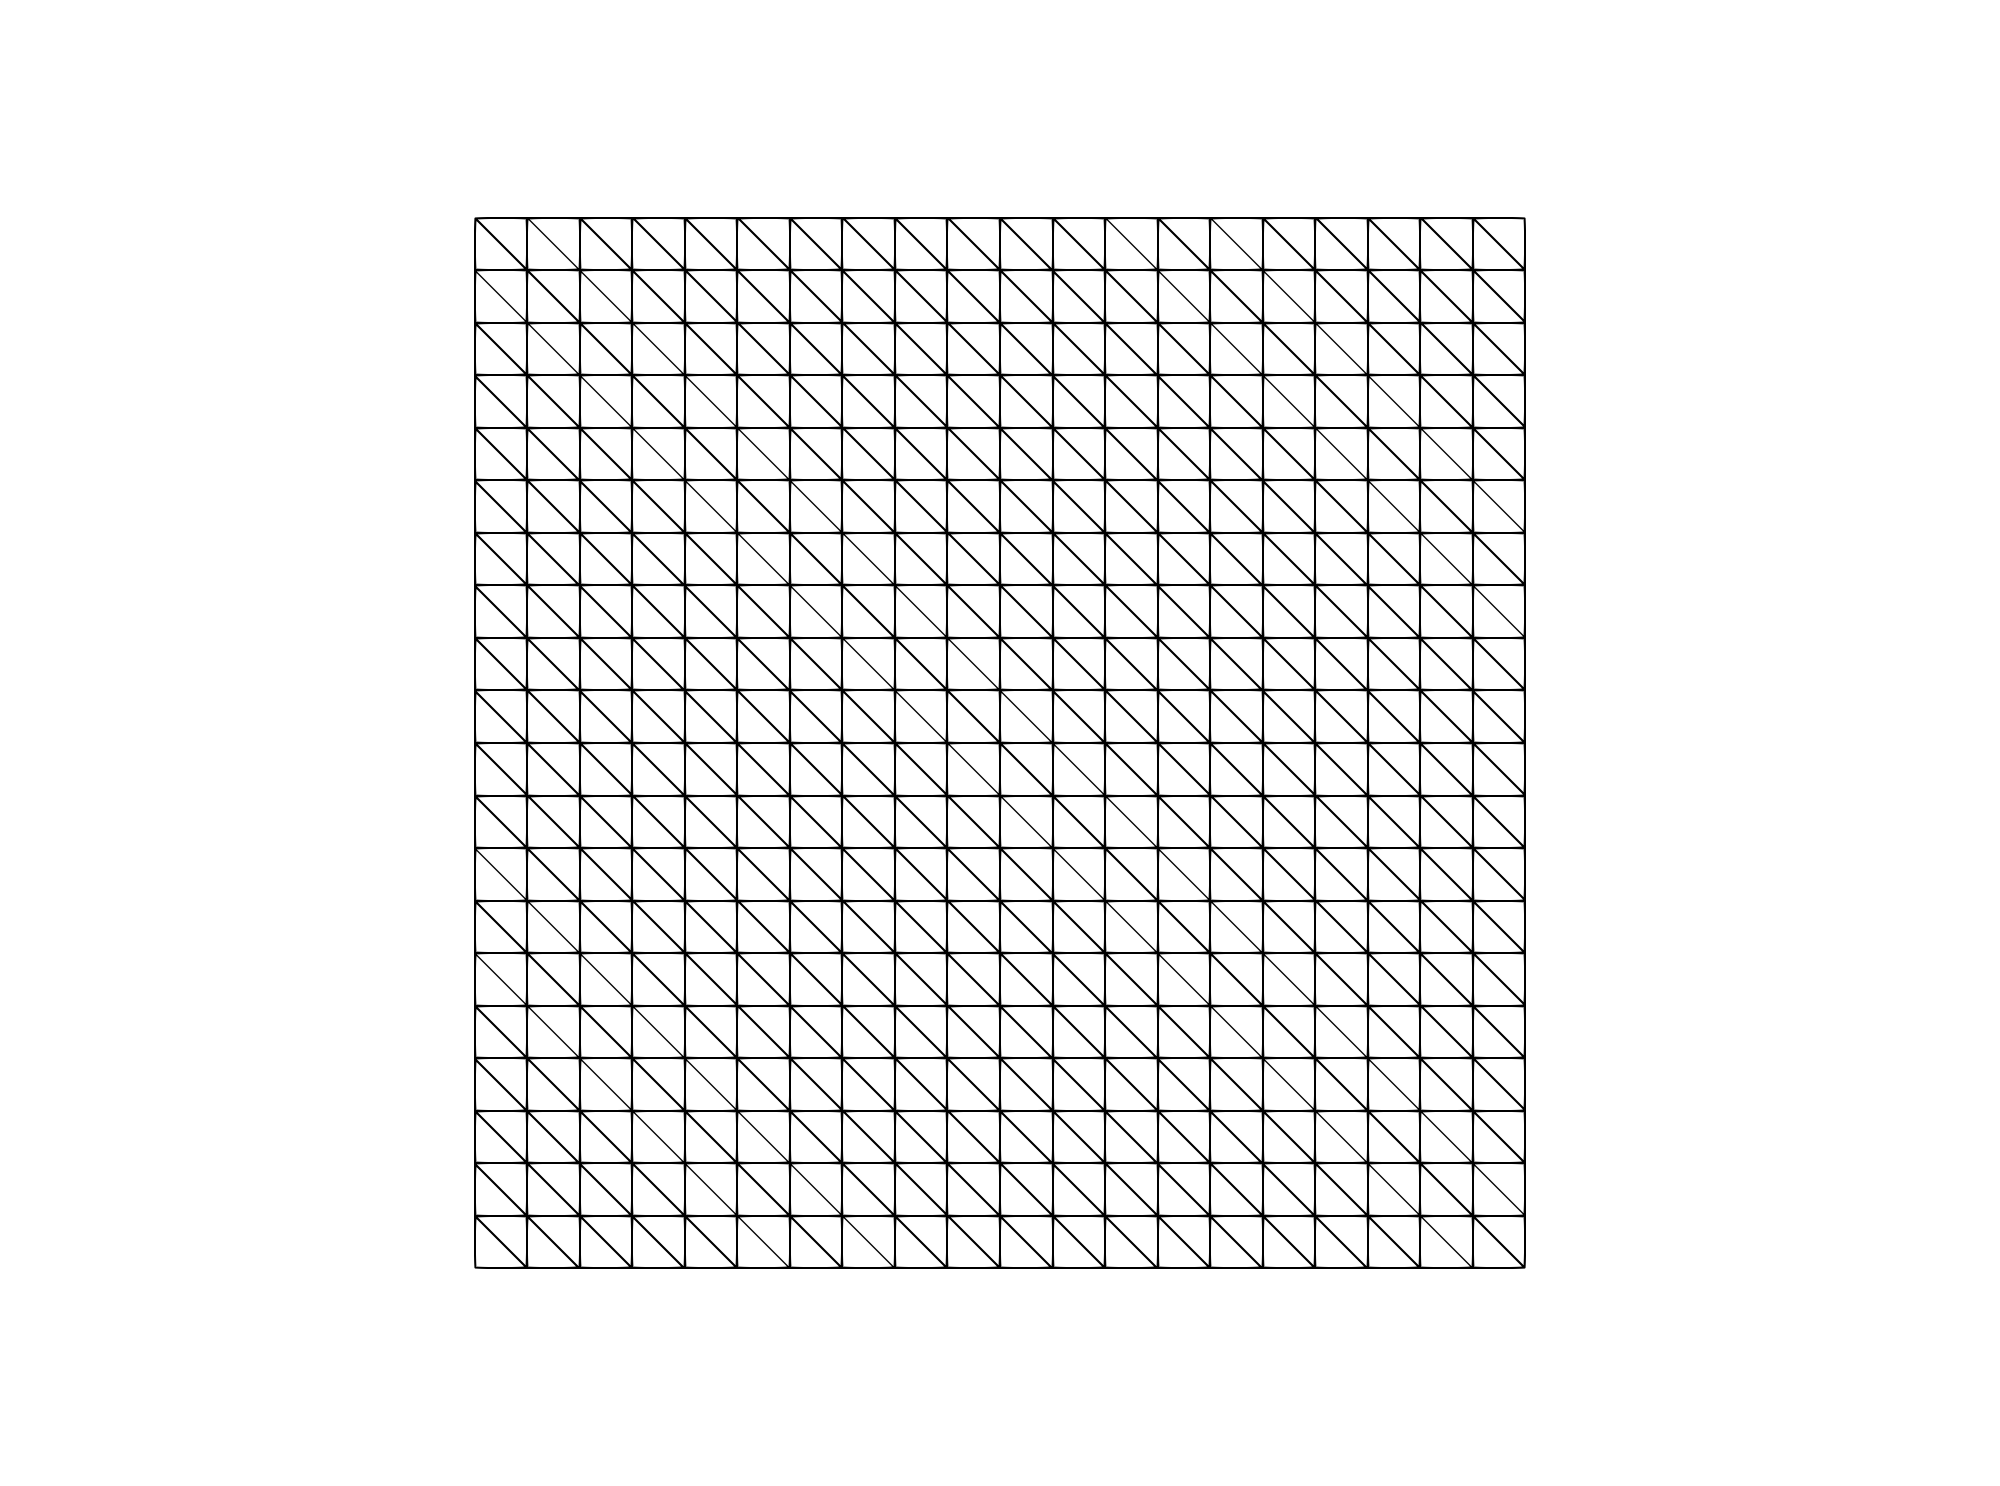
\includegraphics[scale=0.15,trim=9cm 3cm 9cm 6cm, clip=true]{Imagens/Cap5/cav2d_malha_global.png}}
	\label{fig:cav2d_discretização}
	\legend{Fonte: Elaborada pela autora}
\end{figure}

Definiu-se uma espessura para a zona de superposição equivalente a $\delta = 0,1$ e medida paralelamente ao contorno fictício local $(\Gamma_{L})_{B}$. As células pertencentes à zona de superposição na malha local podem ser vistos na Figura~\ref{fig:cav2d_elementos_zs_local}.

\begin{figure}[!htbp]
	\caption{Cavidade 2D: Zona de superposição}
	\centering
	{\includegraphics[scale=1.4, trim=2cm 0.5cm 2cm 0.5cm, clip=true]{Imagens/Cap5/cav2d_elementos_zs_local.pdf}} 
	\label{fig:cav2d_elementos_zs_local}
	\legend{Fonte: Elaborada pela autora}
\end{figure}

Os campos de velocidade e pressão obtidos são apresentados nas Figura~\ref{fig:cav2d_campo_velocidade} e Figura~\ref{fig:cav2d_campo_pressao}. Os perfis de velocidade adimensionalizados ($\velocity/\velocinfty$) horizontal e vertical ao longo de duas linhas centrais nas direções $y_1$ e $y_2$ da cavidade são apresentados na Figura~\ref{fig:cav2d_perfil_vel_Re100} e comparados com os resultados de \citeonline{GhiaGS:1982}.

\begin{figure}[!htbp]
	\caption{Cavidade 2D: Solução do problema de Navier Stokes para $Re = 100$}
	\centering
	\subfloat[\label{fig:cav2d_campo_velocidade} Campo de Velocidade]{\includegraphics[scale=0.21, trim=0cm 0cm 0cm 0cm, clip=true]{Imagens/Cap5/cav2d_campo_vel.pdf}} 
	\subfloat[\label{fig:cav2d_campo_pressao} Campo de Pressão ]{\includegraphics[scale=0.47,trim=3cm 3cm 6cm 3cm, clip=true]{Imagens/Cap5/cav2d_campo_pressao.pdf}}
	\legend{Fonte: Elaborada pela autora}
\end{figure}

\begin{figure}[!!htbp]
	\caption{Cavidade 2D: Perfis de velocidade} 
	\centering
	{\includegraphics[scale=0.8,trim=0cm 0cm 0cm 0cm, clip=true]{Imagens/Cap5/cav2d_perfil_vel_Re100.pdf}}\\
	{\includegraphics[scale=1.0,trim=0cm 0cm 0cm 0cm, clip=true]{Imagens/Cap5/cav2d_legenda.pdf}}
	\label{fig:cav2d_perfil_vel_Re100}
	\legend{Fonte: Elaborada pela autora}
\end{figure}